\documentclass[10pt,a4paper,]{report}

\usepackage[utf8]{inputenc}
\usepackage{amsmath}
\usepackage{amsfonts}
\usepackage{amssymb}
\usepackage{float}
\usepackage{graphicx}
\usepackage{listings}
\usepackage{color}

\author{Nicholas J Shindler}
\title{Machine Learning: Lab 1}

\definecolor{mygreen}{rgb}{0,0.6,0}
\definecolor{mygray}{rgb}{0.92,0.92,0.92}
\definecolor{mymauve}{rgb}{0.58,0,0.82}
\lstset{
	language=Matlab,
	breaklines=true,
	breakatwhitespace=false,
	backgroundcolor=\color{mygray}
}
\hoffset = 0cm
\oddsidemargin = 0.5cm
\textwidth = 420pt

\begin{document}

\maketitle
\tableofcontents

\section*{Part 1}

\lstinputlisting[firstline=61, lastline=65]{lab1.m}

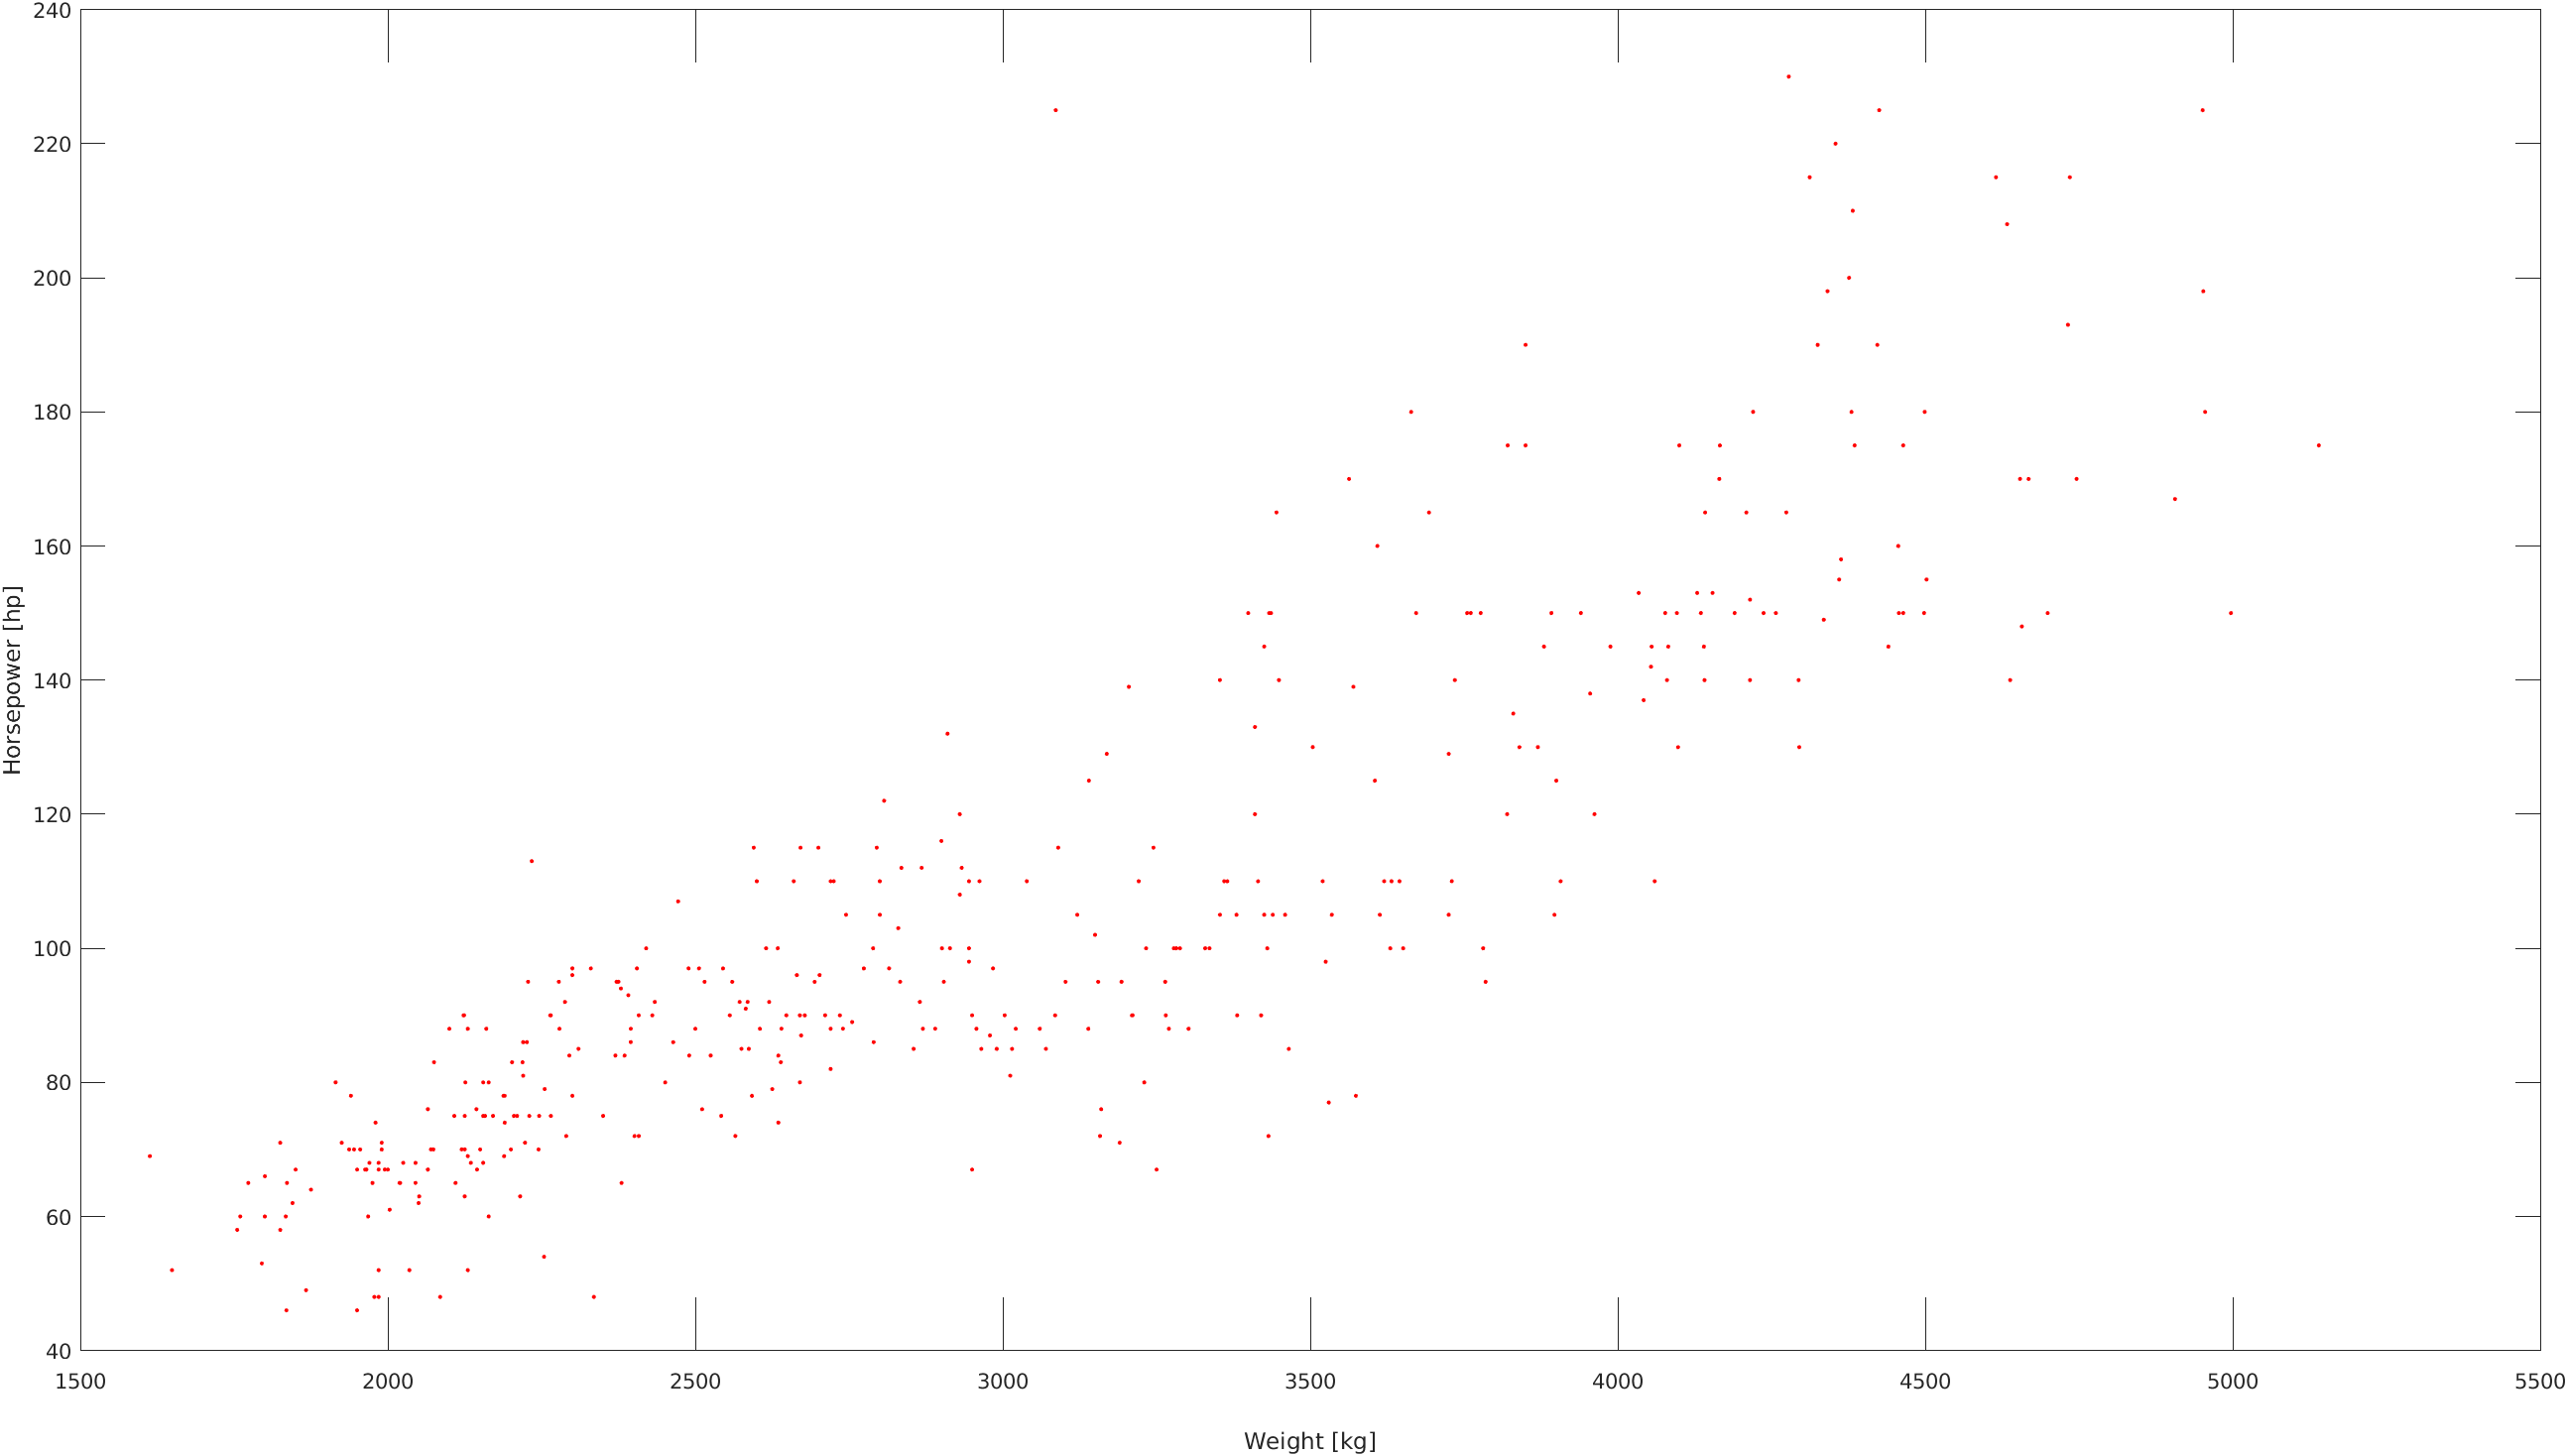
\includegraphics[width=\textwidth]{part1a_hp_v_kg.png}

\lstinputlisting[firstline=81, lastline=87]{lab1.m}

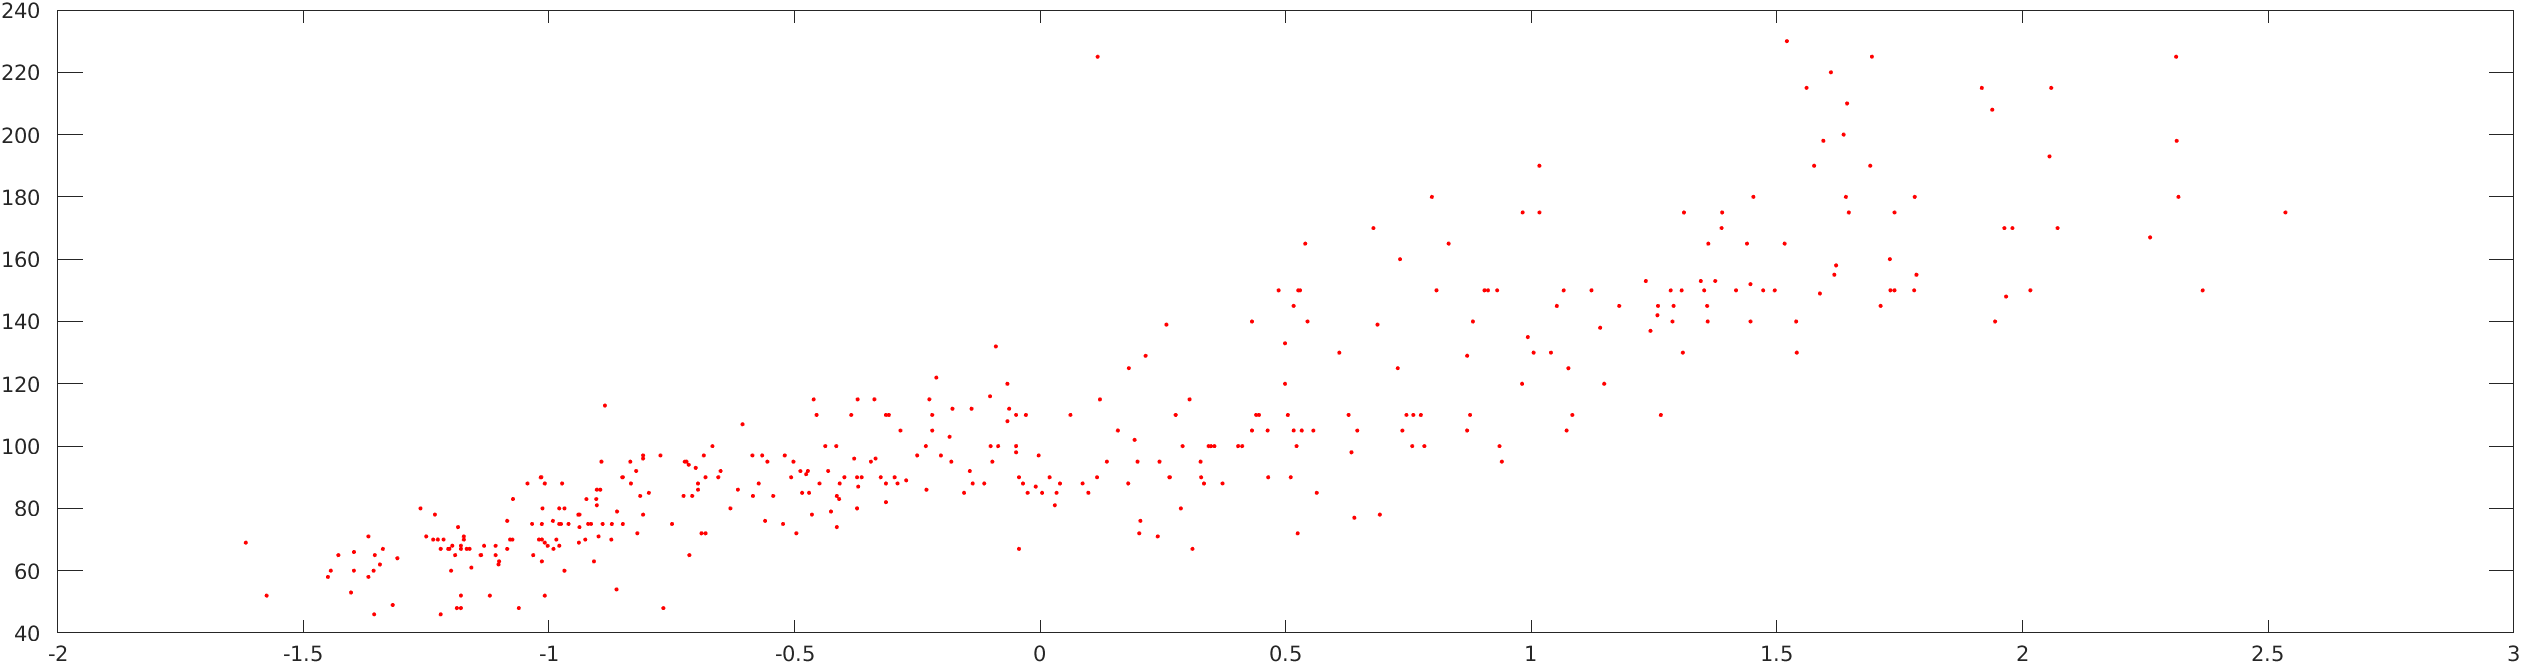
\includegraphics[width=\textwidth]{part1_normalized.png}

\section*{Part 2}
\lstinputlisting[firstline=107, lastline=110]{lab1.m}

\section*{Part 3}

\lstinputlisting[firstline=140, lastline=150]{lab1.m}

\begin{figure}[H]
\label{Gradient decent}
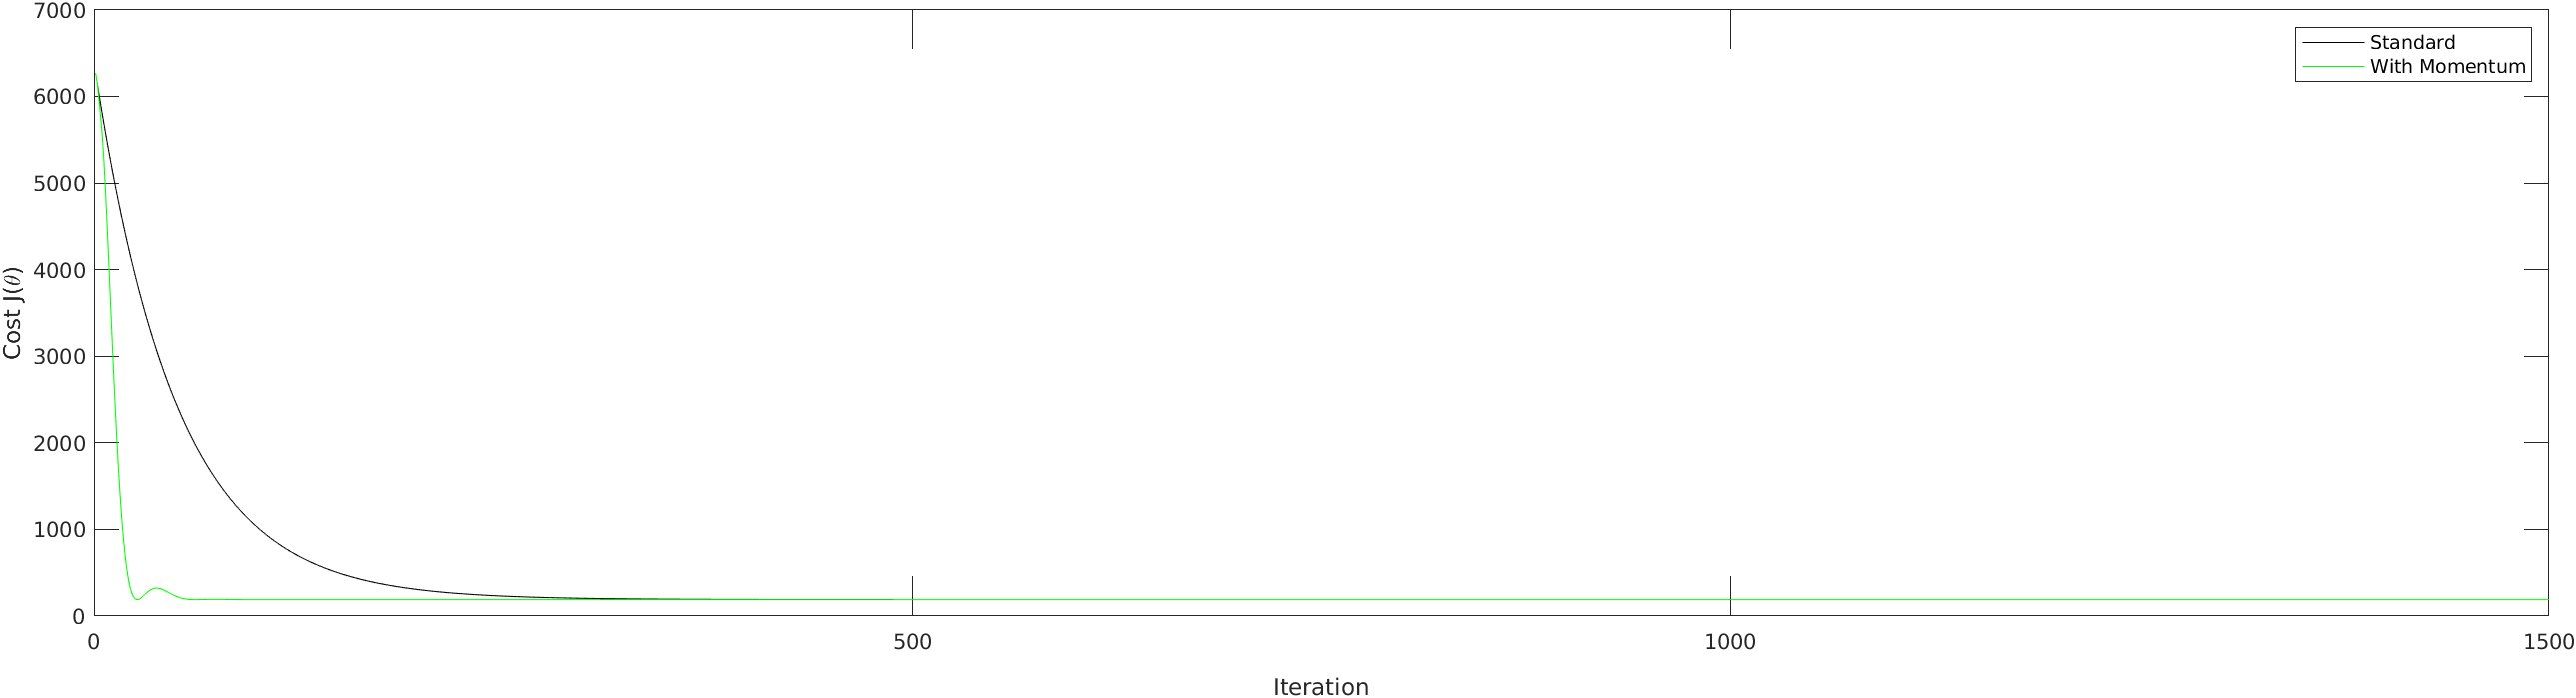
\includegraphics[width=\textwidth]{part3_momentum.png}
\caption{Gradient decent}
\end{figure}
\begin{figure}[H]
\label{Linear regression}
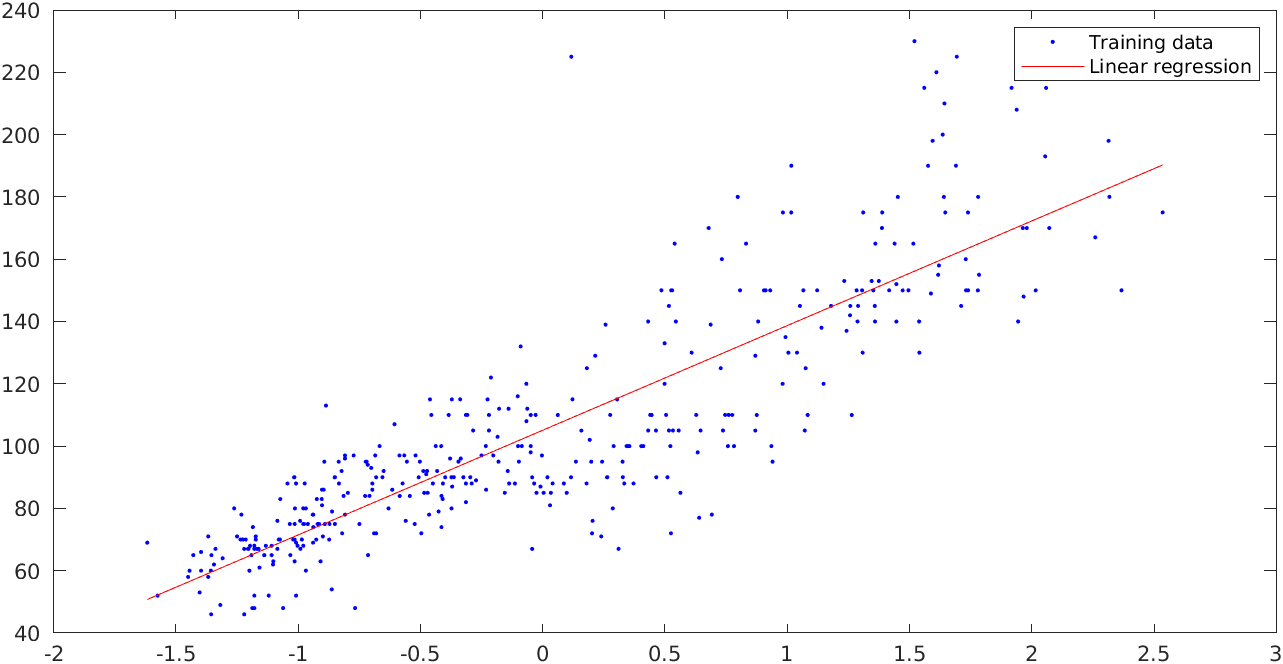
\includegraphics[width=\textwidth]{grad_decent_linreg.png}
\caption{Linear regression}
\end{figure}
\begin{figure}[H]
\label{Linear regression with momentum}
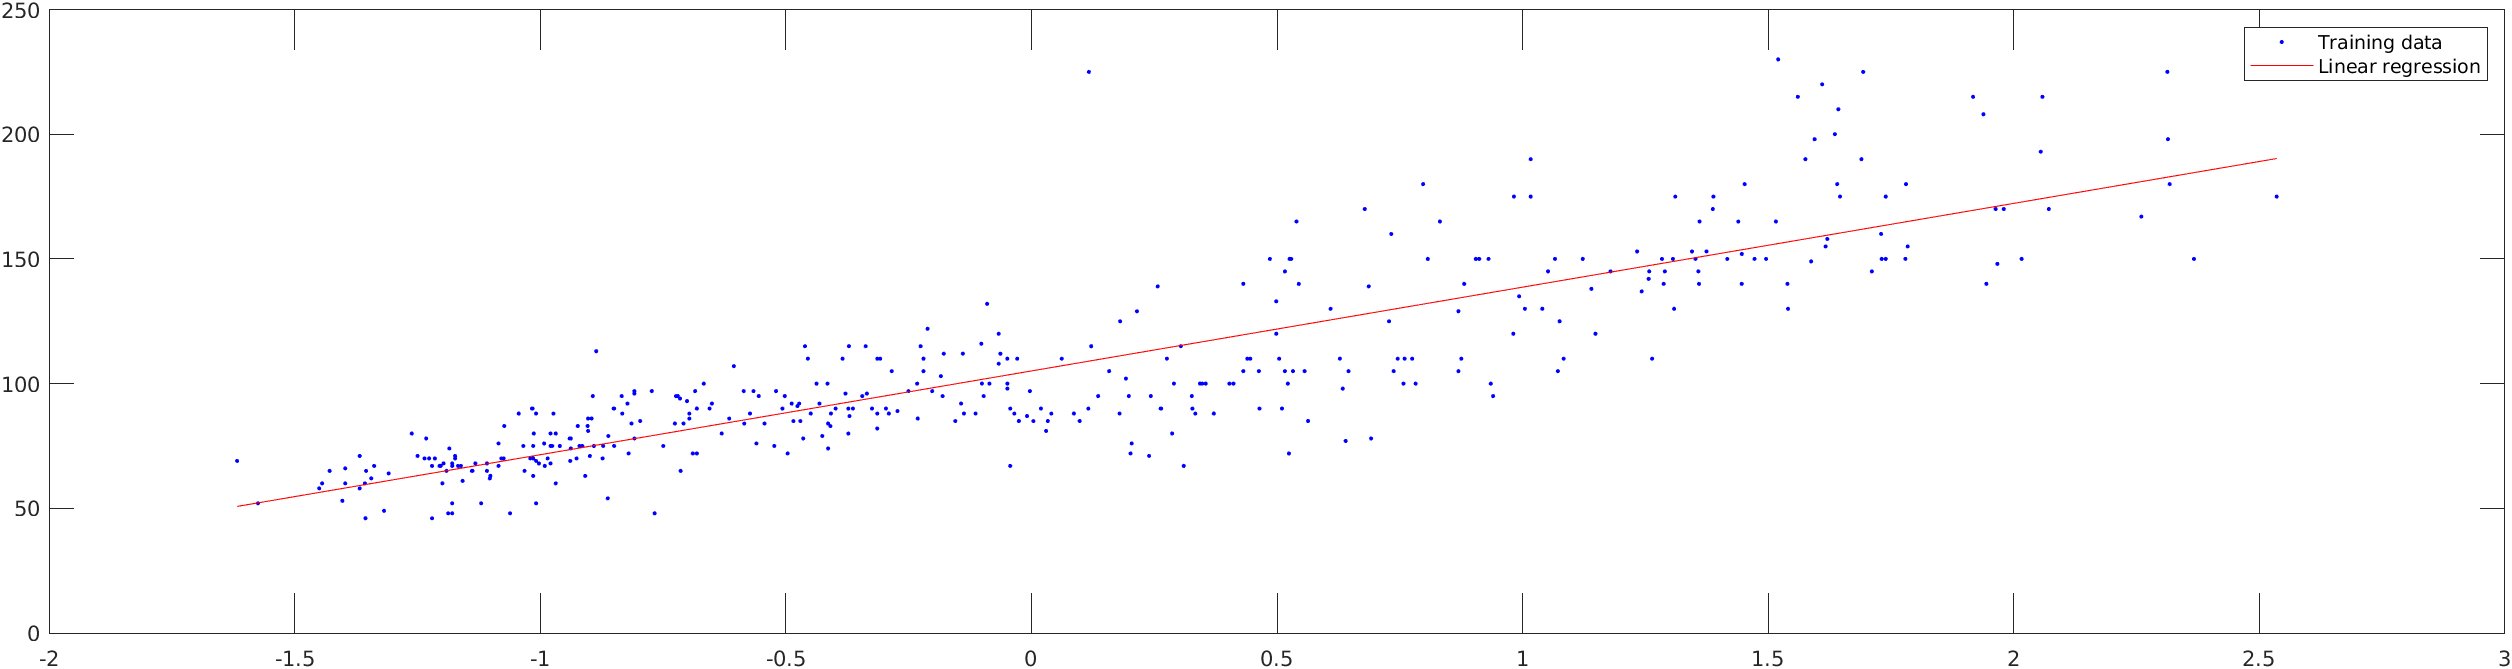
\includegraphics[width=\textwidth]{grad_decent_momentum_linreg.png}
\caption{Linear regression with momentum}
\end{figure}



\end{document}